% !TEX root = ../thesis.tex

%%%%%%%%%%%%%%%%%%%%%%%%%%%%%%%%%%%%%%%%%%%%%%%%%%%%%%%%%%%%%%%%%%%%%%%%%%%%%%%
% Chapter: Metrics Results
%%%%%%%%%%%%%%%%%%%%%%%%%%%%%%%%%%%%%%%%%%%%%%%%%%%%%%%%%%%%%%%%%%%%%%%%%%%%%%%
\chapter{Metrics Results}\label{Metrics Results}

\section{JHotDraw Results}

\subsection{FigureSelectionListener}

\begin{table}[H]
\centering
\resizebox{\textwidth}{!}{%
	\begin{tabular}{@{}lccccccccc@{}}
	\toprule
	\textbf{} & \multicolumn{2}{c}{\textbf{Coupling}} & \textbf{Cohesion} & \multicolumn{3}{c}{\textbf{Size}} & \multicolumn{3}{c}{\textbf{Separation of Concerns}} \\ \midrule
	\textbf{Class} & \textbf{CBC} & \textbf{DIT} & \textbf{LCOO} & \textbf{WOC} & \textbf{LOC} & \textbf{NOA} & \textbf{CDC} & \textbf{CDO} & \textbf{CDLOC} \\
	DrawingView (Subject) & - & - & - & - & 54 & - & 1 & 2 & - \\
	StandardDrawingView (concrete Subject) & 35 & 5 & 17 & 136 & 629 & 21 & 1 & 9 & 20 \\
	NullDrawingView (concrete Subject) & 18 & 5 & 46 & 54 & 155 & 5 & 1 & 2 & 2 \\
	FigureSelectionListener  (Observer) & - & - & - & - & 4 & - & 1 & 1 & - \\
	DrawingEditor  (Interface) & - & - & - & - & 14 & - & 1 & 1 & - \\
	DrawApplication (concrete Observer) & 71 & 6 & 2 & 144 & 726 & 20 & 1 & 1 & 4 \\
	AbstractCommand (concrete Observer) & 33 & 1 & 6 & 28 & 133 & 4 & 1 & 3 & 8 \\
	UndoableCommand (concrete Observer) & 13 & 1 & 4 & 21 & 78 & 3 & 1 & 2 & 12 \\ \bottomrule
	\end{tabular}}
\caption{JHotDraw FigureSelectionListener Metrics}
\label{tbl:JHotDraw FigureSelectionListener Metrics}
\end{table}

\begin{table}[H]
\centering
\resizebox{\textwidth}{!}{%
	\begin{tabular}{@{}lcccccccccc@{}}
	\toprule
	 & \multicolumn{2}{c}{\textbf{Coupling}} & \textbf{Cohesion} & \multicolumn{4}{c}{\textbf{Size}} & \multicolumn{3}{c}{\textbf{Separation of Concerns}} \\ \midrule
	 & \textbf{CBC} & \textbf{DIT} & \textbf{LCOO} & \textbf{WOC} & \textbf{LOC} & \textbf{NOA} & \textbf{VS} & \textbf{CDC} & \textbf{CDO} & \textbf{CDLOC} \\
	\textbf{Total} & 170 & 18 & 75 & 383 & 1793 & 53 & 8 & 8 & 21 & 46 \\
	\textbf{Max} & 71 & 6 & 46 & 144 & 726 & 21 & - & - & 9 & 20 \\
	\textbf{Min} & 13 & 1 & 2 & 21 & 4 & 3 & - & - & 1 & 2 \\
	\textbf{Average} & 34 & 3.6 & 15 & 76.6 & 224.125 & 10.6 & - & - & 2.625 & 9.2 \\ \bottomrule
	\end{tabular}}
\caption{JHotDraw FigureSelectionListener Totals}
\label{tbl:JHotDraw FigureSelectionListener Totals}
\end{table}

\subsection{ChangeAttributeCommand}

\begin{table}[H]
\centering
\resizebox{\textwidth}{!}{%
	\begin{tabular}{@{}lcccccccccc@{}}
	\toprule
	\textbf{} & \multicolumn{2}{c}{\textbf{Coupling}} & \textbf{Cohesion} & \multicolumn{3}{c}{\textbf{Size}} & \multicolumn{3}{c}{\textbf{Separation of Concerns}} \\ \midrule
	\textbf{Class} & \textbf{CBC} & \textbf{DIT} & \textbf{LCOO} & \textbf{WOC} & \textbf{LOC} & \textbf{NOA} & \textbf{CDC} & \textbf{CDO} & \textbf{CDLOC} \\
	Command & - & - & - & - & 12 & - & 1 & 2 & - \\
	AbstractCommand & 33 & 1 & 6 & 28 & 133 & 4 & 1 & 4 & 12 \\
	UndoableCommand & 13 & 1 & 4 & 21 & 78 & 3 & 1 & 2 & 4 \\
	ChangeAttributeCommand & 11 & 2 & 2 & 5 & 103 & 2 & 1 & 3 & 6 \\
	DrawApplication & 71 & 6 & 2 & 144 & 726 & 20 & 1 & 5 & 10 \\ \bottomrule
	\end{tabular}}
\caption{JHotDraw ChangeAttributeCommand Metrics}
\label{tbl:JHotDraw ChangeAttributeCommand Metrics}
\end{table}

\begin{table}[H]
\centering
\resizebox{\textwidth}{!}{%
	\begin{tabular}{@{}lcccccccccc@{}}
	\toprule
	 & \multicolumn{2}{c}{\textbf{Coupling}} & \textbf{Cohesion} & \multicolumn{4}{c}{\textbf{Size}} & \multicolumn{3}{c}{\textbf{Separation of Concerns}} \\ \midrule
	 & \textbf{CBC} & \textbf{DIT} & \textbf{LCOO} & \textbf{WOC} & \textbf{LOC} & \textbf{NOA} & \textbf{VS} & \textbf{CDC} & \textbf{CDO} & \textbf{CDLOC} \\
	\textbf{Total} & 128 & 10 & 14 & 198 & 1052 & 29 & 5 & 5 & 16 & 32 \\
	\textbf{Max} & 71 & 6 & 6 & 144 & 726 & 20 & - & - & 5 & 12 \\
	\textbf{Min} & 11 & 1 & 2 & 5 & 12 & 2 & - & - & 2 & 4 \\
	\textbf{Average} & 32 & 2.5 & 3.5 & 49.5 & 210.4 & 7.25 & - & - & 3.2 & 8 \\ \bottomrule
	\end{tabular}}
\caption{JHotDraw ChangeAttributeCommand Totals}
\label{tbl:JHotDraw ChangeAttributeCommand Totals}
\end{table}

% \section{AJHotDraw Results}

\section{ManagedDataJHotDraw Results}

\subsection{FigureSelectionListener}

\begin{table}[H]
\centering
\resizebox{\textwidth}{!}{%
	\begin{tabular}{@{}lccccccccc@{}}
	\toprule
	\textbf{} & \multicolumn{2}{c}{\textbf{Coupling}} & \textbf{Cohesion} & \textbf{Size} & \textbf{} & \textbf{} & \multicolumn{3}{c}{\textbf{Separation of Concerns}} \\ \midrule
	\textbf{Class / Data manager} & \textbf{CBC} & \textbf{DIT} & \textbf{LCOO} & \textbf{WOC} & \textbf{LOC} & \textbf{NOA} & \textbf{CDC} & \textbf{CDO} & \textbf{CDLOC} \\
	MDDrawingView (Interface) & - & - & - & - & 111 & - & 0 & 0 & 0 \\
	MDStandardDrawingView (Managed Data) & 26 & 2 & 16 & 120 & 471 & 18 & 0 & 0 & 0 \\
	MDNullDrawingView (Managed Data) & 15 & 2 & 31 & 38 & 120 & 8 & 0 & 0 & 0 \\
	MDDrawingViewFactory (Helper) & 17 & 1 & 1 & 8 & 177 & - & 1 & 1 & 0 \\
	DrawingViewSchemaFactory (SchemaFactory) & - & - & - & - & 4 & 0 & 0 & 0 & 0 \\
	FigureSelectionListenerMObject (Data Manager) & 5 & 3 & 4 & 6 & 28 & 0 & 1 & 4 & 0 \\
	DrawingEditor  (Interface) & - & - & - & - & 12 & - & 0 & 0 & - \\
	DrawApplication (concrete Observer) & 72 & 6 & 2 & 145 & 732 & 20 & 1 & 1 & 2 \\
	AbstractCommand (concrete Observer) & 33 & 1 & 6 & 28 & 133 & 4 & 0 & 0 & 0 \\
	UndoableCommand (concrete Observer) & 16 & 1 & 4 & 23 & 90 & 3 & 1 & 2 & 4 \\ \bottomrule
	\end{tabular}}
\caption{MDJHotDraw FigureSelectionListener Metrics}
\label{tbl:MDJHotDraw FigureSelectionListener Metrics}
\end{table}

\begin{table}[H]
\centering
\resizebox{\textwidth}{!}{%
	\begin{tabular}{@{}lccccccccc@{}}
	\toprule
	 & \multicolumn{2}{c}{\textbf{Coupling}} & \textbf{Cohesion} & \multicolumn{3}{c}{\textbf{Size}} & \multicolumn{3}{c}{\textbf{Separation of Concerns}} \\ \midrule
	 & \textbf{CBC} & \textbf{DIT} & \textbf{LCOO} & \textbf{WOC} & \textbf{LOC} & \textbf{NOA} & \textbf{CDC} & \textbf{CDO} & \textbf{CDLOC} \\
	\textbf{Total} & 184 & 16 & 64 & 368 & 1878 & 53 & 4 & 8 & 6 \\
	\textbf{Max} & 72 & 6 & 31 & 145 & 732 & 20 & - & 4 & 4 \\
	\textbf{Min} & 5 & 1 & 1 & 6 & 4 & 0 & - & 0 & 0 \\
	\textbf{Average} & 26.285 & 2.285 & 9.142 & 52.571 & 187.8 & 7.571 & - & 0.8 & 0.66 \\ \bottomrule
	\end{tabular}}
\caption{MDJHotDraw FigureSelectionListener Totals}
\label{tbl:MDJHotDraw FigureSelectionListener Totals}
\end{table}

\subsection{ChangeAttributeCommand}

\begin{table}[H]
\centering
\resizebox{\textwidth}{!}{%
	\begin{tabular}{@{}lcccccccccc@{}}
	\toprule
	 & \multicolumn{2}{c}{\textbf{Coupling}} & \textbf{Cohesion} & \multicolumn{4}{c}{\textbf{Size}} & \multicolumn{3}{c}{\textbf{Separation of Concerns}} \\ \midrule
	\textbf{Class / Data manager} & \textbf{CBC} & \textbf{DIT} & \textbf{LCOO} & \textbf{WOC} & \textbf{LOC} & \textbf{NOA} & \textbf{VS} & \textbf{CDC} & \textbf{CDO} & \textbf{CDLOC} \\
	Command & - & - & - & - & 10 & - & 1 & 0 & - & 0 \\
	AbstractCommand & 33 & 1 & 6 & 28 & 133 & 4 & 1 & 0 & 0 & 0 \\
	UndoableCommand & 16 & 1 & 3 & 23 & 90 & 3 & 1 & 1 & 1 & 2 \\
	UndoableChangeAttrCmdMObject & 7 & 3 & 1 & 3 & 98 & 0 & 1 & 1 & 2 & 0 \\
	DrawApplication & 72 & 6 & 2 & 145 & 732 & 20 & 1 & 1 & 5 & 10 \\ \bottomrule
	\end{tabular}}
\caption{MDJHotDraw ChangeAttributeCommand Metrics}
\label{tbl:MDJHotDraw ChangeAttributeCommand Metrics}
\end{table}

\begin{table}[H]
\centering
\resizebox{\textwidth}{!}{%
	\begin{tabular}{@{}lcccccccccc@{}}
	\toprule
	\multicolumn{1}{c}{\textbf{}} & \multicolumn{2}{c}{\textbf{Coupling}} & \textbf{Cohesion} & \multicolumn{4}{c}{\textbf{Size}} & \multicolumn{3}{c}{\textbf{Separation of Concerns}} \\ \midrule
	\multicolumn{1}{c}{\textbf{}} & \textbf{CBC} & \textbf{DIT} & \textbf{LCOO} & \textbf{WOC} & \textbf{LOC} & \textbf{NOA} & \textbf{VS} & \textbf{CDC} & \textbf{CDO} & \textbf{CDLOC} \\
	\textbf{Total} & 128 & 11 & 12 & 199 & 1063 & 27 & 5 & 3 & 8 & 12 \\
	\textbf{Max} & 72 & 6 & 6 & 145 & 732 & 20 & - & - & 5 & 10 \\
	\textbf{Min} & 7 & 1 & 1 & 3 & 10 & 0 & - & - & 0 & 0 \\
	\textbf{Average} & 32 & 2.75 & 3 & 49.75 & 212.6 & 6.75 & - & - & 2 & 2.4 \\ \bottomrule
	\end{tabular}}
\caption{MDJHotDraw ChangeAttributeCommand Totals}
\label{tbl:MDJHotDraw ChangeAttributeCommand Totals}
\end{table}

\section{Metrics Comparison Graphs}\label{Metrics Comparison Graphs}

\subsection{FigureSelectionListener}

\begin{figure}[H]
	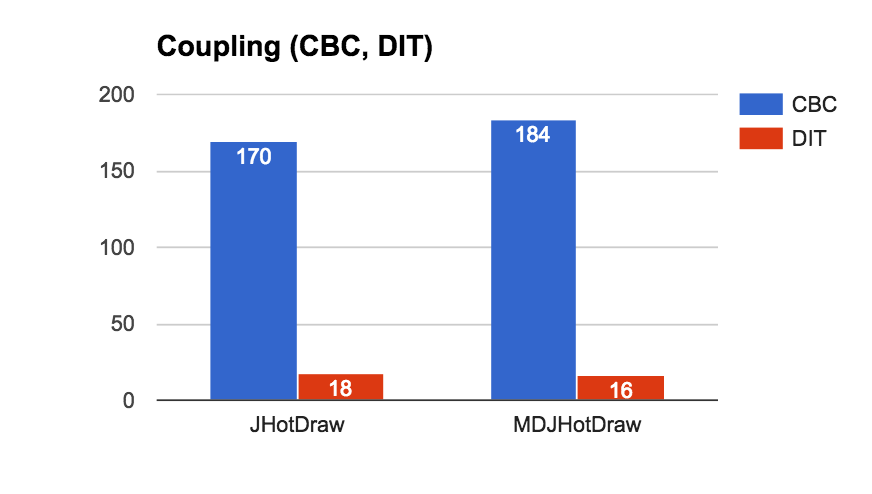
\includegraphics[scale=0.5]{figures/metrics/Metric_Observer_Coupling.png}
	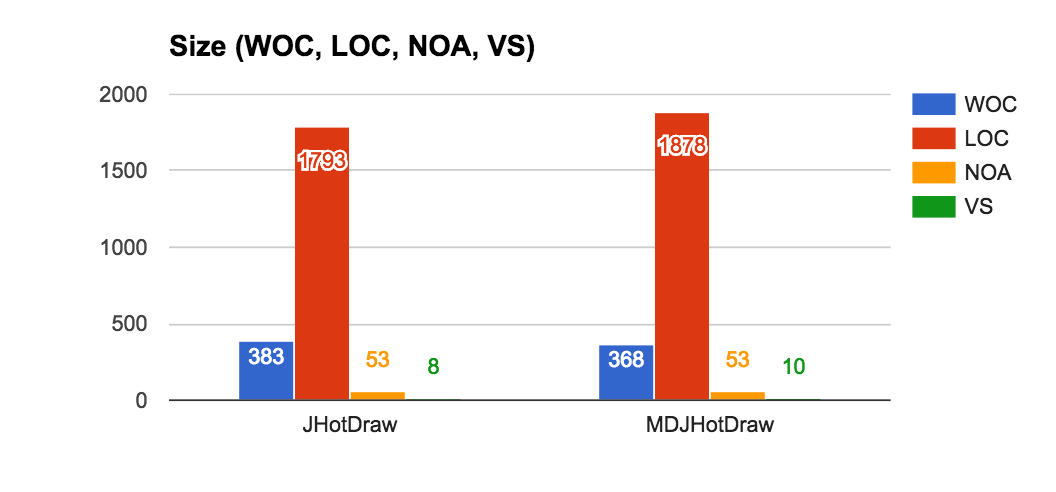
\includegraphics[scale=0.45]{figures/metrics/Metric_Observer_Size.png}

	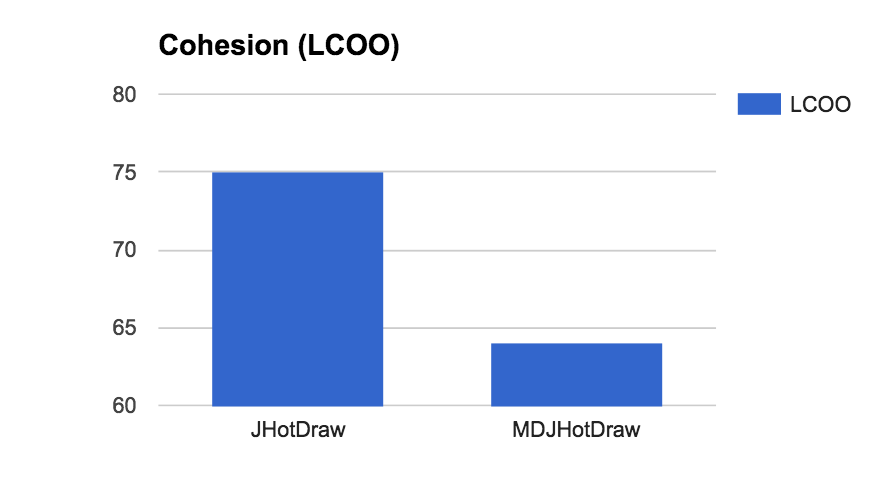
\includegraphics[scale=0.5]{figures/metrics/Metric_Observer_Cohesion.png}
	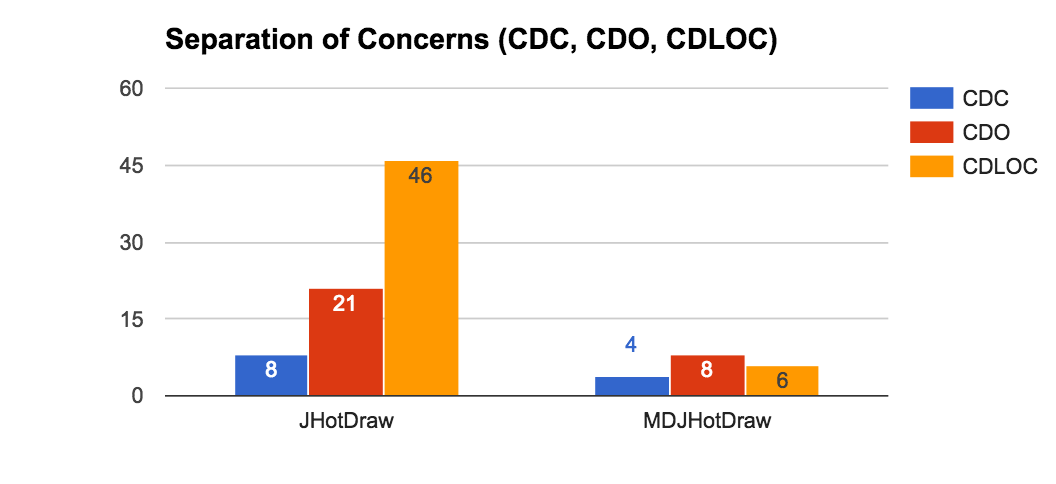
\includegraphics[scale=0.45]{figures/metrics/Metric_Observer_SoC.png}
	\caption{FigureSelectionListener Graphs}
	\label{Fig:FigureSelectionListener Graphs}
\end{figure}

\subsection{ChangeAttributeCommand}

\begin{figure}[H]
	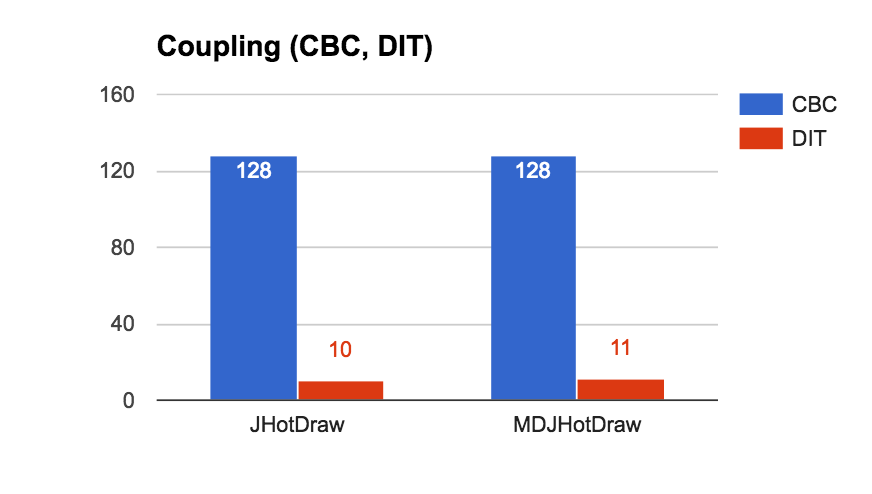
\includegraphics[scale=0.5]{figures/metrics/Metric_Undo_Coupling.png}
	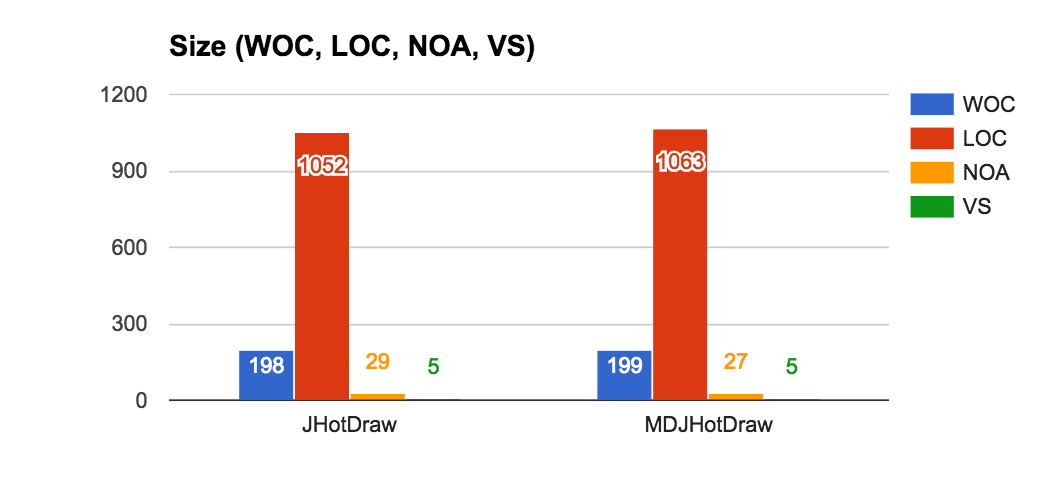
\includegraphics[scale=0.45]{figures/metrics/Metric_Undo_Size.png}

	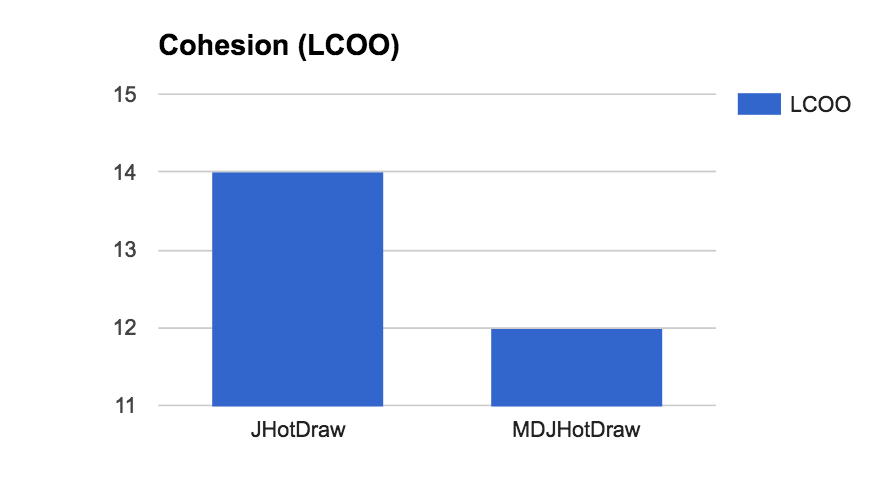
\includegraphics[scale=0.5]{figures/metrics/Metric_Undo_Cohesion.png}
	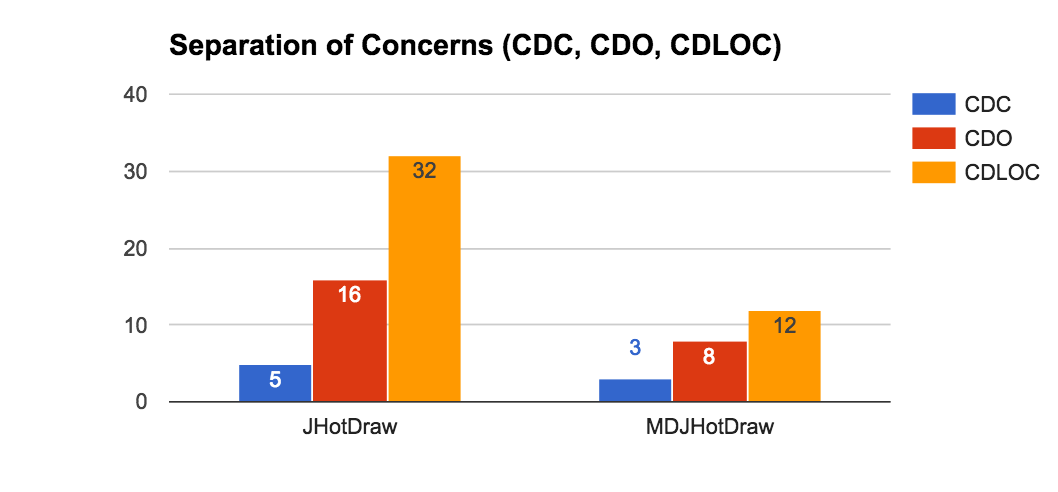
\includegraphics[scale=0.45]{figures/metrics/Metric_Undo_SoC.png}
	\caption{ChangeAttributeCommand Graphs}
	\label{Fig:ChangeAttributeCommand Graphs}
\end{figure}
